\chapter{Transaktionen im Bitcoin-Netzwerk}\label{chp:transaktion-im-bitcoin-netzwerk}
Um nun einen konkreten Anwendungsfalls einer Transaktion in einem Blockchain-Netzwerk zu erläutern, wird darauf eingegangen, wie eine Bitcoin-Transaktion abläuft und welche Bestandteile eine Transaktion besitzt.

Zuerst muss jedoch klargestellt werden, dass bei Bitcoin keine klassischen Kontostände wie bei einem herkömmlichen Konto einer Bank existieren. Der ``Kontostand'' einer Bitcoin-Adresse wird anhand von allen vergangenen Transaktionen der Blockchain ermittelt. Soll also der Saldo einer Bitcoin-Adresse ermittelt werden, muss über die komplette Blockchain iteriert und alle beteiligten Transaktionen summiert werden \footnote{\parencite[vgl.][]{BTCACADEMY.08.03.2021}}.

\section{Bestandteile einer Transaktion}\label{sec:bestandteile-einer-transaktion}
Eine Transaktion im Bitcoin-Netzwerk besteht immer aus mindestens einem \textbf{Input}, mehreren \textbf{Outputs} und einer \textbf{Ziel-} und \textbf{Absender-Adresse}. Um einen Input in einer Transaktion anzugeben, muss bei der Absender-Adresse ein sogenannter ``Unspent Transaction Output'' (UTXO) hinterlegt sein. Dieser wiederum ist ein Output einer vorher getätigten Transaktion. Sobald einer Person nach einer Transaktion ein UTXO in Form eines Outputs einer früheren Transaktion gutgeschrieben wurde, kann diese ihn benutzen und an andere Personen schicken \footnote{\parencite[vgl.][]{entwickler.de.NaN}}. 

Jedoch muss dabei beachtet werden, dass die UTXOs nicht aufgeteilt werden können. Hat Person A beispielsweise einen UTXO in Höhe von 1 BTC, will jedoch nur 0.5 BTC an Person B schicken, muss Person A bei der Transaktion ein ``Rückgeldkonto'' anlegen, zu dem die Differenz der beiden Beträge transferiert wird. Wird dieses Konto nicht angegeben, erhält der Miner die Differenz zwischen dem Input und dem Output einer Transaktion \footnote{\parencite[vgl.][]{BTCACADEMY.08.03.2021}}. 

\begin{figure}[h]
    \begin{centering}
        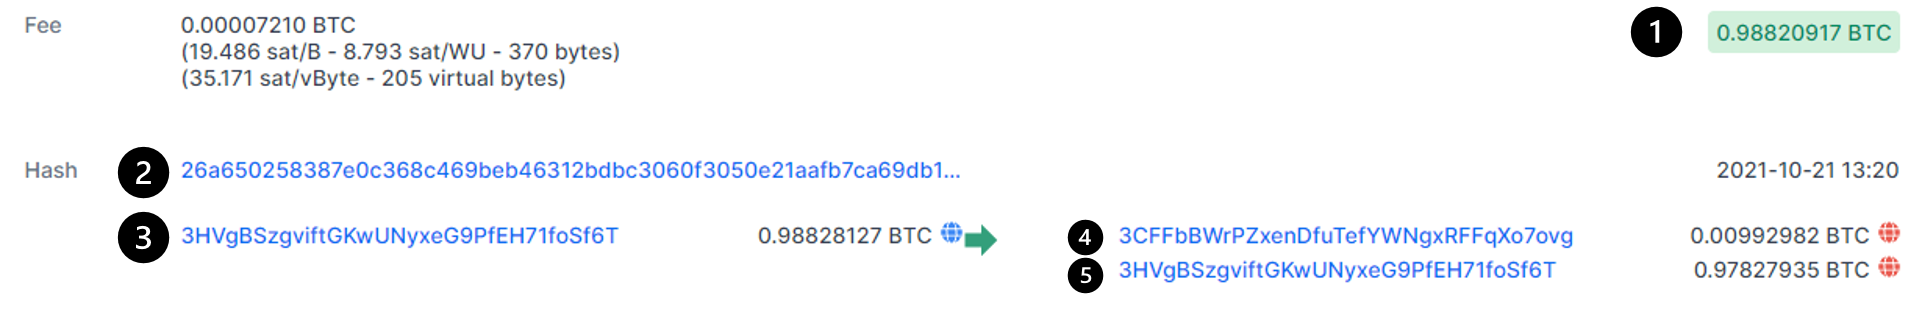
\includegraphics[width=1.1\linewidth]{Transaktion.png}
        \caption[Transaktion eines Blocks]{Transaktion eines Blocks \footnotemark}
        \label{fig:transaktion}
    \end{centering}
\end{figure}
\footnotetext{\parencite[vgl.][]{.27.10.2021}}

In \vref{fig:transaktion} ist ein solches Vorgehen abgebildet. Bei der Transaktion 2 sendet die Absenderadresse 3 etwa 0.9882 BTC (1) an die Zieladresse 4. Da der UTXO 1 jedoch 0.9882 BTC beträgt und nur etwa 0.0099 BTC an die Zieladresse 4 gesendet werden soll, wird der Rest erneut als Output an die Absenderadresse 5 transferiert, welches dem Wallet entspricht, von dem der Input der Transaktion kam.


\section{Locking Script und Unlocking Script}\label{sec:locking-unlocking}
